El objetivo principal de este capítulo es describir una extensión del método propuesto por \cite{FerYosWas18} que permita evaluar la seguridad de un sistema que ha sido construido usando patrones de seguridad. En la primera sección se describe a grandes rasgos los elementos necesarios para realizar la evaluación. En las secciones posteriores se detalla cómo identificar las amenazas, la evaluación propuesta y la interpretación del resultado obtenido. 

\vspace{0.3cm}

Cada sección es ejemplificada utilizando el caso de uso de un sistema financiero básico denominado \textit{Auditoría de órdenes de comercio}.

\section{Descripción general del método}

En la Figura \ref{diagramabase} se muestra el diagrama a bloques que representa los elementos de la evaluación propuesta. Se describen a grandes rasgos cada elemento, siendo los tres primeros bloques (requisitos de seguridad, patrones de seguridad y casos de uso) los elementos obtenidos del sistema a evaluar que denominaremos previos requeridos, el elemento de amenazas y por último los elementos evaluación de seguridad y resultado que son en los que se enfoca el desarrollo de este trabajo. 

\begin{figure}[h!]
\centering
	\begin{tikzpicture}
		\node (fig1) at (0,0) {\includegraphics[scale=0.7]{Imagenes/diag_block_method.eps}};
		%\node (fig2) at (5,-3) {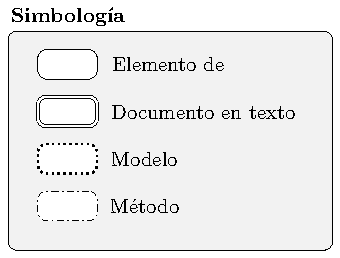
\includegraphics[scale=0.5]{Imagenes/simDiagrama1.eps}};
	\end{tikzpicture}
\caption{Diagrama a bloques.}
\label{diagramabase}
\end{figure}

\subsection*{Previos requeridos}

Dado que el presente trabajo se enfoca en evaluar un sistema construido utilizando patrones de seguridad en el diseño, los previos requeridos son obtenidos tanto del modelo UML como de la documentación que exista sobre el sistema. 

\begin{itemize}
	\item \textbf{Requisitos de seguridad}. Se considera que el sistema tiene varios requisitos de seguridad, obtenidos de un listado de políticas de seguridad, políticas internas de la empresa o políticas gubernamentales. \\
	Cada requisito de seguridad tiene una prioridad diferente para la empresa, usando dos niveles:
	\begin{itemize}[noitemsep]
		\item \textbf{Baja}. Cubrir el requisito de seguridad es deseable.
		\item \textbf{Alta}. Cubrir el requisito de seguridad es imprescindible. 
	\end{itemize}
	Por ejemplo, los requisitos de seguridad correspondientes a \textit{Auditoría de órdenes de comercio} .
	\begin{itemize}[noitemsep]
		\item $Req_1$. Se debe tener registro de todos los inicios de sesión realizados por el auditor (\textit{prioridad baja}). 
		\item $Req_2$. Se deben registrar todas las acciones realizadas por el auditor (\textit{prioridad alta}).
		\item $Req_3$. El auditor solo puede leer la información de ordenes (asignadas a él) (\textit{prioridad alta}).
		%\item $Req_4$. El auditor puede verificar las transacciones relacionadas a una orden asignada a él (\textit{prioridad alta}).
	\end{itemize}
	\item \textbf{Casos de uso}. Los casos de uso definen las posibles interacciones de usuarios con el sistema e indican las actividades y la información que se está manipulando en el sistema que se ha desarrollado.\\
	La Tabla \ref{CU5_descripcion} muestra el resumen de la documentación correspondiente al caso de uso \textit{Auditoría de órdenes de comercio}. 
	
	\begin{table}[!ht]
		\caption{Resumen auditoría de órdenes de comercio}
		\begin{center}
		\scriptsize{
		\begin{tabular}{ |m{1.5cm}|m{1cm}|m{7cm}|}
		\hline
		\cellcolor{lightgray}\textbf{CU-5} & \multicolumn{2}{|c|}{\cellcolor{lightgray}\textbf{Auditoría de órdenes de comercio}} \\\hline
		Pre-condición & \multicolumn{2}{m{8cm}|}{El auditor debe tener un listado de órdenes de comercio ya finalizadas.} \\\hline
		Descripción & \multicolumn{2}{m{8cm}|}{El sistema debe comportarse como se describe en el siguiente caso de uso cuando el auditor solicite inspeccionar una orden.}\\\hline
		\multirow{3}{1.5cm}{Secuencia normal} & Paso& Acción\\\cline{2-3}
		&1& El auditor solicita al sistema realizar la inspección de una orden de comercio.\\\cline{2-3}
		&2& El auditor inspecciona la orden de comercio con respecto a las regulaciones gubernamentales y de la empresa.\\\cline{2-3}
		&3& El auditor genera un informe tomando en cuenta el análisis realizado a la orden de comercio.\\\hline
		Post-condición&\multicolumn{2}{m{8cm}|}{El auditor genera el informe de la orden de comercio.}\\\hline
		Excepciones & Paso & Acción \\ \cline{2-3}
		&4 & El auditor de tener más ordenes de comercio asignadas a él repetirá los pasos del 1 al 3.\\\hline
		Comentarios & \multicolumn{2}{m{8cm}|}{ El auditor solo puede revisar las ordenes de comercio asignadas a él.} \\\hline
		
		\end{tabular}
		}
		\end{center}
		\label{CU5_descripcion}
	\end{table}
	
	La Figura \ref{ej_useCase_actDiag} muestra los diagramas correspondiente al caso de uso \textit{Auditoría de órdenes de comercio}. 

	\begin{figure}[h!]
	\begin{center}
   		\subfloat[Caso de uso]{ \label{useCase_check}
    			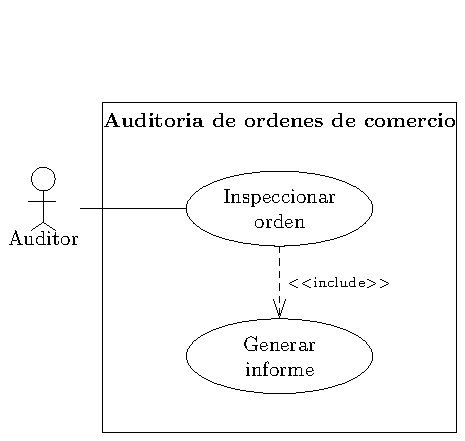
\includegraphics[width=0.4\textwidth]{Imagenes/diag_useCase_checkTrade_esp.eps}}
    			\hspace{1cm}
  		\subfloat[Diagrama de actividades]{ \label{actDiag_check}
    			\includegraphics[width=0.3\textwidth]{Imagenes/diag_activity_checkTrade_esp.eps}}
 		\caption{Caso de uso: Auditoría de ordenes de comercio}
 		\label{ej_useCase_actDiag}
 	\end{center}
	\end{figure}
	\item \textbf{Patrones de seguridad}. Los patrones de seguridad son los que han sido implementados en el sistema y que provienen de algún catálogo pre-especificado.\\
		A continuación se indican los patrones correspondientes al caso de uso \textit{Auditoría de órdenes de comercio}:
	\begin{itemize}[noitemsep]
		\item $Pat_1$: Role-based access control
		\item $Pat_2$: Authenticator
		\item $Pat_3$: Security logger and auditor
	\end{itemize}
	En este previo requerido se pueden encontrar de la misma manera patrones de regulación y roles\footnote{Los patrones de regulación se encuentran en desarrollo, por lo que para ciertos sistemas deben escribirse patrones para completar los diagramas, es decir, hace falta contar con un catálogo de patrones de regulación como catálogo de patrones de seguridad.}.
\end{itemize}


\subsection*{Modelado de amenazas}

Una vez que contamos con los previos requeridos, se procede a hacer el análisis de amenazas a las que está expuesto el sistema. Para este proceso, por cada caso de uso se obtiene el conjunto de amenazas.

\vspace{0.3cm}

Todas las amenazas obtenidas por cada caso de uso son consideradas para el presente trabajo como, el total de amenazas a las que está expuesto el sistema. Por ello es importante usar métodos de enumeración sistemáticos que garanticen la identificación de las amenazas importantes.


\subsection*{Evaluación de seguridad del sistema}

La evaluación de seguridad conjunta tanto los requisitos de seguridad (que son las metas de seguridad que se han planteado para el sistema) como las amenazas a las que está expuesto el sistema que se ha desarrollado. Dado que el sistema fue construido utilizando patrones de seguridad, estos mitigarán ciertas amenazas proporcionando un nivel de seguridad al mismo. 

\vspace{0.3cm}

La evaluación contempla que no todas las amenazas tienen el mismo impacto en el sistema y por ello se puede prescindir de evitar las de menor impacto. 

\subsection*{Resultado de la evaluación: métrica de seguridad}

Una vez aplicado el método de evaluación al sistema, se obtiene un valor el cual indica qué tan seguro es el sistema ante las amenazas identificadas considerándolo como el resultado de la evaluación. Se da una interpretación a los diferentes posibles resultados, que van desde no hacer nada más a agregar nuevas defensas. 

\section{Modelado de amenazas}\label{cap4:sec:ModAme}

Para el método propuesto, se ha agregado una columna a la tabla creada en \cite{BraFerVan08}. La columna \textbf{Impacto} define el impacto que tiene dicha amenaza en el sistema a criterio de la empresa, usando tres niveles:

\begin{itemize}[noitemsep]
	\item \textbf{Bajo}. La amenaza de existir genera un riesgo insignificante para la empresa.
	\item \textbf{Medio}. La amenaza tiene un impacto en la empresa pero no es crítica. 
	\item \textbf{Alto}. La amenaza es considerada de alto impacto para la empresa y crítica.
\end{itemize}

Este nuevo criterio nos permite dar un peso diferente a las amenazas a las que está expuesto el sistema. Una determinada amenaza puede ser de mayor impacto para un sistema que para otro dependiendo de el contexto en el que se implemente; es decir, obtener la información de cuenta de un usuario de banco es diferente a obtener los tuits de un usuario en un foro.

\vspace{0.3cm}

Las amenazas son obtenidas por cada caso de uso del sistema, por lo tanto, en la columna \# de la tabla se coloca como abreviatura $T_{ca}$, donde la \textbf{T} proviene de la palabra en inglés (\textit{Threat}), \textbf{c} es el número de actividad analizada y \textbf{a} es el número de amenaza dentro de la actividad.

\vspace{0.3cm}

La Tabla \ref{misAct_ex} muestra la plantilla de actividades de mal uso con los datos requeridos del análisis de amenazas\footnote{Atri. seg. es la abreviatura dada a Atributo de Seguridad/Objetivo de Seguridad en el presente trabajo.}. 

\begin{table}[!ht]
\caption{Plantilla de actividades de mal uso}
\begin{center}
\scriptsize{
\begin{tabular}{ |m{1cm}|m{1.5cm}|m{0.5cm}|m{0.5cm}|m{1.3cm}|m{1cm}|m{1.7cm}|m{1cm}|}
\hline
	\cellcolor{lightgray}\textbf{Actor} &\cellcolor{lightgray} \textbf{Actividad} & \cellcolor{lightgray}\textbf{\#} &\cellcolor{lightgray} \textbf{Atri. seg.} &\cellcolor{lightgray}\textbf{Impacto} & \cellcolor{lightgray}\textbf{Origen ataque} &\cellcolor{lightgray} \textbf{Descripción} &\cellcolor{lightgray} \textbf{Activo} \\ \hline
	&&&&&&&\\\hline
\end{tabular}
}
\end{center}
\label{misAct_ex}
\end{table}

Se realiza el análisis de amenazas utilizando el método de \cite{BraFerVan08} con las modificaciones descritas anteriormente para el caso de uso \textit{Auditoría de órdenes de comercio} y utilizando el diagrama de actividades mostrado en la Figura \ref{actDiag_check}.

\vspace{0.3cm}

Para comenzar con la búsqueda de amenazas, existen tres posibles atacantes u origen de la amenaza (Interno autorizado, Interno no autorizado, Externo no autorizado) y por cada actividad se considera \textit{``¿Qué mal uso se puede realizar en <actividad> por el <origen de amenaza> que compromete el <atributo de seguridad> del <dato a proteger>''} como se muestra a continuación:

\begin{itemize}[noitemsep]
	\item ¿Qué mal uso se puede realizar en \textit{Inspeccionar Orden} por el \textit{Auditor} que compromete la \textit{Responsabilidad} sobre el \textit{Informe} ?: Negar haber inspeccionado una orden.
	\item ¿Qué mal uso se puede realizar en \textit{Inspeccionar Orden} por \textit{Auditor} que compromete la \textit{Confidencialidad} de la \textit{Orden}? : Copiar la información de la orden para otros usos e inspeccionar órdenes no asignadas a él. 
	\item ¿Qué mal uso se puede realizar después de haber \textit{Inspeccionado todas las ordenes} por el \textit{Auditor/Impostor} que compromete la \textit{Responsabilidad} sobre el \textit{Informe} ?: Enviar información a una persona externa a la empresa.
	\item ¿Qué mal uso se puede realizar en \textit{Generar Informe} por el \textit{Auditor/Impostor} que compromete la \textit{Responsabilidad} del \textit{Informe}? : Ignorar los requerimientos gubernamentales o de la empresa.
	\item ¿Qué mal uso se puede realizar en \textit{Generar Informe} por el \textit{Atacante externo} que compromete la \textit{Confidencialidad} del \textit{Informe}? : Leer la información del informe generado.
\end{itemize} 

Con el análisis anterior se llena la tabla modificada de actividades de mal uso, identificando el impacto que tiene cada una en la empresa como se muestra en la Tabla \ref{resModAme}, también se puede visualizar este análisis de una forma gráfica como se muestra en la Figura \ref{diag_malUso}.

\begin{table}[!ht]
\caption{Resultado de amenazas Auditoría de órdenes de comercio}
\begin{center}
\scriptsize{
\begin{tabular}{ |P{1cm}|m{1.5cm}|c|P{0.5cm}|c|P{1cm}|m{6cm}|c|}
\hline
	\cellcolor{lightgray}\textbf{Actor} &\cellcolor{lightgray} \textbf{Actividad} & \cellcolor{lightgray}\textbf{\#} &\cellcolor{lightgray} \textbf{Atri. seg.}&\cellcolor{lightgray}\textbf{Impacto} & \cellcolor{lightgray}\textbf{Origen ataque} &\cellcolor{lightgray} \centering \textbf{Descripción} &\cellcolor{lightgray} \textbf{Activo} \\ \hline
	\multirow{2}{*}{\centering Auditor} &\multirow{2}{*}{\shortstack[l]{ Inspeccionar \\ Orden}} & T$_{1_1}$ & R &Bajo& InA & Negar haber inspeccionado una orden de compra & Orden \\ \cline{3-8}
	 &  & T$_{1_2}$ & C& Alto & InA/InN & Copiar información de ordenes para otros usos & Orden \\ \hline
	 \multirow{3}{*}{\centering Auditor }& \multirow{3}{*}{\shortstack[l]{Generar \\ Informe}}& T$_{2_1}$ & R & Alto& InA & Ignorar los reglamentos gubernamentales o de la empresa aplicables a una orden al generar un informe & Informe \\ \cline{3-8}
	 &  & T$_{2_2}$ & R & Alto & InA  & Enviar información de los informes a una persona externa & Informe \\ \cline{3-8}
	& & T$_{2_3}$ & C& Medio & Ext  & Leer información sobre los informes generados & Informe \\ \hline
\end{tabular}
}
\label{resModAme}
\end{center}
\end{table}

\begin{figure}[!ht]
\begin{center}
	\begin{tikzpicture}
		\node (fig1) at (0,0) {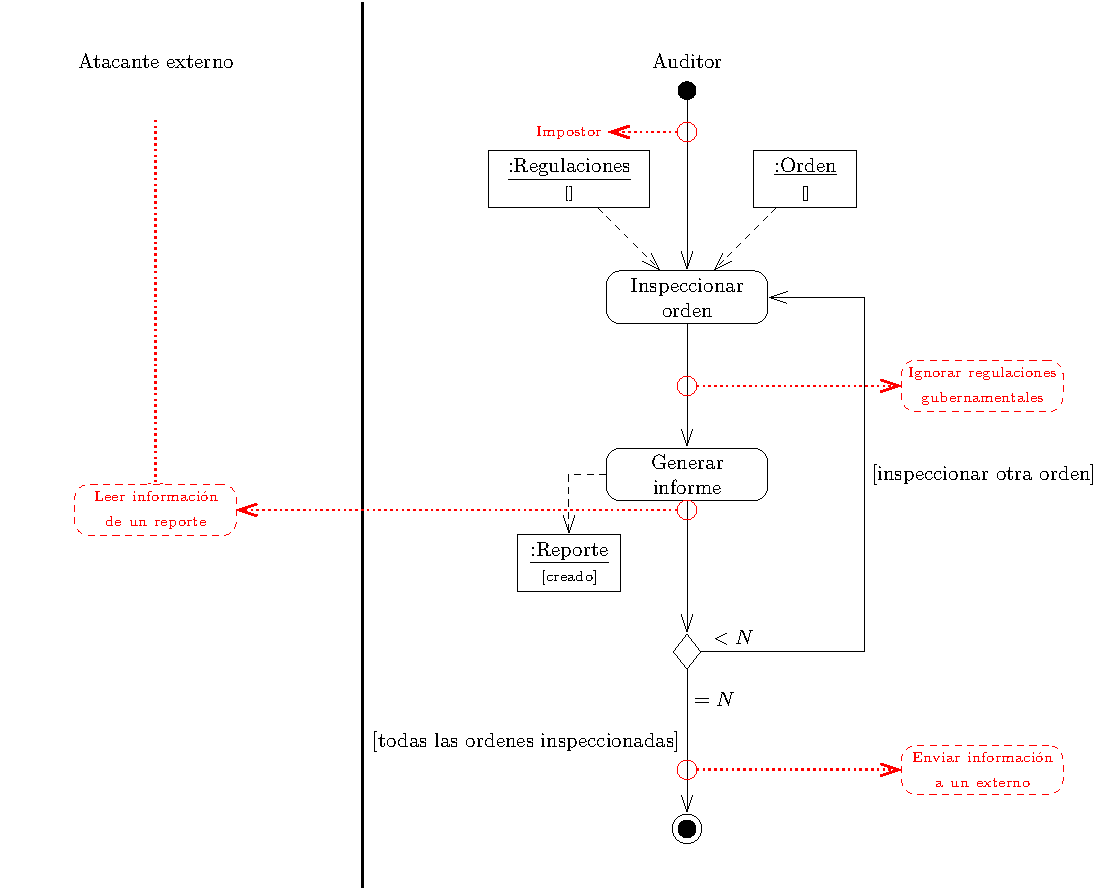
\includegraphics[scale=0.7]{Imagenes/diag_activity_checkTrade_misuse_esp.eps}};
		\node (fig2) at (5.5,4) {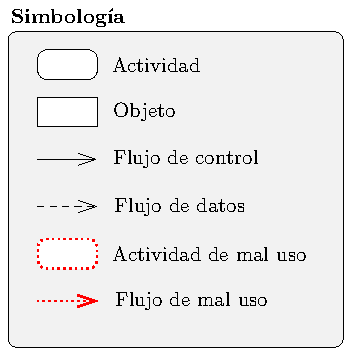
\includegraphics[scale=0.5]{Imagenes/simAct_diag_check_trade.eps}};
	\end{tikzpicture}
\end{center}
\caption{Diagrama con actividades de mal uso}
\label{diag_malUso}
\end{figure}



\section{Método de evaluación de seguridad} 


\begin{enumerate}[label=Paso \arabic*:,leftmargin=*]
\setcounter{enumi}{0}
%Paso 1 del método
\item Se debe encontrar el peso de las amenazas mitigadas sobre el sistema, representado como $w_{ame}$. Para este paso se cuenta con tres fases:

\begin{enumerate}[noitemsep]
	\item Se relaciona cada patrón de seguridad con la amenaza que mitiga, si el patrón mitiga más de una amenaza debe replicarse en cada una. En caso de existir al menos un patrón se asigna un valor de $v_p=1$ que indica que existe una mitigación de la amenaza\footnote{Este valor no indica que la amenaza desaparece.}, si no existe al menos un patrón que mitigue la amenaza se asigna un valor de $v_p=0$ indicando que dicha amenaza persiste.
	 
	\item Esta siguiente fase nos permite conocer el impacto de las amenazas sobre el sistema. Para esta fase a cada nivel de impacto se le asigna un valor: \textbf{Bajo=1}, \textbf{Medio=2}, \textbf{Alto=3}.
	
	\vspace{0.3cm}
	
	Cada amenaza tiene un valor de impacto en el sistema como:
	
	\begin{equation*}
		\alpha= \frac{imp}{M}
	\end{equation*}
 
 	Donde, $\alpha$ es el peso de la amenaza; $imp$ es el impacto de la amenaza y $M$ es el número total de amenazas identificadas. 
 
	\item Por último, para obtener los pesos de las amenazas mitigadas se utiliza:
	
	\begin{equation*}
		w_{ame}= \frac{\displaystyle\sum_{i=1}^{M}\alpha_i \cdot v_{p_i}}{\displaystyle\sum_{i=1}^{M}\alpha_i} \hspace{30pt} (0 \leq w_{ame} \leq 1)
	\end{equation*}
	
	Donde, $w_{ame}$ es peso mitigado para el sistema, $\alpha_i$ es el peso de cada amenaza y $v_{p_i}$ es el valor de patrón asignado a la amenaza $\alpha_i$.

\end{enumerate}

La Tabla \ref{datos_eval_ame} muestra la plantilla de impacto de amenazas con la información obtenida del paso anterior. 

\begin{table}[!ht]
\caption{Plantilla de datos impacto de amenazas}
\begin{center}
\scriptsize{
\begin{tabular}{ |c|c|c|c|c|}
\hline
	\cellcolor{lightgray}Amenaza&\cellcolor{lightgray}Patrón(es)&\cellcolor{lightgray}$\alpha$& \cellcolor{lightgray}$v_p$ & \cellcolor{lightgray}$w_{ame}$ \\ \hline
	&&&&\\\hline
\end{tabular}
}
\end{center}
\label{datos_eval_ame}
\end{table}

Usando el caso de uso de \textit{Auditoría de ordenes de comercio} y la información obtenida en la Tabla \ref{resModAme} se procede a llenar la tabla del impacto de amenazas como se muestra en la Tabla \ref{eval_ame}.

\begin{table}[!ht]
\caption{Impacto de las amenazas}
\renewcommand{\arraystretch}{1.5}
\begin{center}
\scriptsize{
\begin{tabular}{ |c|c|c|c|c|}
\hline
	\cellcolor{lightgray}Amenaza&\cellcolor{lightgray}Patrón(es)&\cellcolor{lightgray}$\alpha$& \cellcolor{lightgray}$v_p$ & \cellcolor{lightgray}$w_{ame}$ \\ \hline
	T$_1{_1}$&Pat$_3$&$\frac{1}{5}$&1&\multirow{5}{*}{$\frac{\frac{1}{5}\cdot 1+\frac{3}{5}\cdot 1+\frac{3}{5}\cdot 1+\frac{3}{5}\cdot 1+\frac{2}{5}\cdot 1}{\frac{12}{5}}=1$}\\\cline{1-4}
	T$_1{_2}$&Pat$_1$&$\frac{3}{5}$&1&\\\cline{1-4}
	T$_2{_1}$&Pat$_3$&$\frac{3}{5}$&1&\\\cline{1-4}
	T$_2{_2}$&Pat$_1$&$\frac{3}{5}$&1&\\\cline{1-4}
	T$_2{_3}$&Pat$_2$&$\frac{2}{5}$&1&\\\hline
\end{tabular}
}
\end{center}
\label{eval_ame}
\end{table}


%Paso dos del método
\item Se debe contar con el peso de los requerimientos de seguridad satisfechos en el sistema tanto por patrones de seguridad como patrones de regulación o roles, representado como $w_{req}$. Para esto se cuenta con las siguientes fases:

\begin{enumerate}[noitemsep]
	\item Se relaciona cada patrón de seguridad, patrón de regulación o rol con el requisito de seguridad que atiende, si el patrón o rol atiende más de un requisito de seguridad debe replicarse en cada una. En caso de existir al menos un patrón se asigna un valor de $v_p=1$ que indica que el requisito de seguridad es satisfecho, si no existe al menos un patrón se asigna un valor de $v_p=0$ indicando que no ha sido atendido.
	\item Conociendo la prioridad que tiene cada requisito de seguridad para la empresa se obtiene el peso de cada uno asignando un valor a cada prioridad: \textbf{Baja}=1,\textbf{Media}=2 \textbf{Alta}=3.\\
	Cada requisito de seguridad tendrá una prioridad en el sistema como:
	\begin{equation*}
		\mu= \frac{prio}{N}
	\end{equation*}
	Donde, $\mu$ es el importancia del requisito de seguridad en el sistema, $prio$ es la prioridad y $N$ es el número total de requisitos de seguridad proporcionados. 
	
	\item Por último, para obtener el peso de todos los requisitos de seguridad satisfechos se utiliza:
	
	\begin{equation*}
		w_{req}= \frac{\displaystyle\sum_{j=1}^{N}\mu_j \cdot v_{p_j}}{\displaystyle\sum_{j=1}^{N}\mu_j} \hspace{30pt} (0 \leq w_{req} \leq 1)
	\end{equation*}
	
	Donde $w_{req}$ es peso de los requisitos de seguridad atendidos en el sistema, $\mu_j$ es la importancia de cada requisito de seguridad y $v_{p_j}$ es el valor de patrón asignado al requisito o política $\mu_j$.
\end{enumerate}

La Tabla \ref{datos_eval_req} muestra la plantilla de los requisitos de seguridad satisfechos con la información obtenida del paso anterior. 

\begin{table}[!ht]
\caption{Plantilla de datos requisitos de seguridad satisfechos}
\begin{center}
\scriptsize{
\begin{tabular}{ |c|c|c|c|c|}
\hline
	\cellcolor{lightgray}Requisito&\cellcolor{lightgray}Patrón(es)&\cellcolor{lightgray}$\mu$& \cellcolor{lightgray}$v_p$ & \cellcolor{lightgray}$w_{req}$ \\ \hline
	&&&&\\\hline
\end{tabular}
}
\end{center}
\label{datos_eval_req}
\end{table}

Usando el caso de uso de \textit{Auditoría de ordenes de comercio} y la información sobre los requisitos de seguridad se procede a llenar la tabla de requisitos de seguridad atendidos como se muestra en la Tabla \ref{eval_req}.

\begin{table}[!ht]
\caption{Requisitos de seguridad satisfechos}
\renewcommand{\arraystretch}{1.5}
\begin{center}
\scriptsize{
\begin{tabular}{ |c|c|c|c|c|}
\hline
	\cellcolor{lightgray}Requisito&\cellcolor{lightgray}Patrón(es)&\cellcolor{lightgray}$\mu$& \cellcolor{lightgray}$v_p$ & \cellcolor{lightgray}$w_{req}$ \\ \hline
	Req$_1$&Pat$_3$&$\frac{1}{4}$&1&\multirow{5}{*}{$\frac{\frac{1}{4}\cdot 1+\frac{2}{4}\cdot 1+\frac{1}{4}\cdot 1+\frac{2}{4}\cdot 1}{\frac{6}{4}}=1$}\\\cline{1-4}
	Req$_2$&Pat$_3$&$\frac{2}{4}$&1&\\\cline{1-4}
	Req$_3$&Pat$_1$&$\frac{1}{4}$&1&\\\cline{1-4}
	Req$_4$&Pat$_1$&$\frac{2}{4}$&1&\\\hline
\end{tabular}
}
\end{center}
\label{eval_req}
\end{table}

\item Se obtiene el total de la seguridad del sistema, definido como :

\begin{equation*}
	ss = w_{ame} \cdot w_{req}
\end{equation*}

Donde, $w_{ame}$ son las amenazas mitigadas por los patrones de seguridad en el sistema y $w_{req}$ son los requisitos de seguridad satisfechos por los patrones de seguridad identificados en el sistema. La multiplicación de ambos pesos indican el nivel de seguridad del sistema $ss$; es decir, definen una métrica que combina seguridad y políticas de la empresa.\\

El valor obtenido también puede ayudar a analizar la seguridad del sistemas y observar dónde es necesario hacer mejoras para incrementar la seguridad del mismo o identificar si existen elementos seguridad que hacen ineficiente al sistema de los cuales se puede prescindir sin perder seguridad.  

\end{enumerate}

\section{Resultado de la evaluación}\label{cap4_sec_Res}

En esta sección se explica la interpretación que debe darse al valor numérico denominado $ss$ obtenido en la sección anterior. 

\vspace{0.3cm}

El valor de seguridad del sistema $ss$ debe encontrarse en el rango de 0 a 1. Si se encuentra cercano al 1 (uno) indica que el sistema está completamente o casi seguro ante las amenazas identificadas y se han satisfecho todos los requisitos de seguridad; en caso contrario, si el valor $ss$ está cercano al 0 (cero) indica que el sistema es propenso a cualquier amenaza y que los requisitos de seguridad no están siendo satisfechos. 

En la Figura \ref{resulss} se muestra una representación de 3 casos en los que el valor $ss$ puede tener una interpretación diferente. 

\begin{figure}[!ht]
  \centering
    \includegraphics[scale=1]{Imagenes/fig_resultSS.eps}
    \caption{Indicador del nivel de seguridad.}
    \label{resulss}
\end{figure}

\begin{itemize}[noitemsep]
\item Cuando el valor $0\ldotp7 < ss \leq 1$ : Al encontrarse dentro de este rango, la interpretación que se da es que al menos para cierta cantidad de amenazas el sistema se encuentra protegido y los requisitos de seguridad están siendo satisfechos. En particular, dentro de este rango el valor de $ss$ al ser 1 indica que el sistema está protegido para las amenazas identificadas; pero pueden existir amenazas no identificadas.
\item Cuando el valor $0\ldotp3 < ss \leq  0\ldotp7$ : Si el valor $ss$ se encuentra dentro de este rango, se puede considerar que el sistema está protegido pero la posibilidad de que exista una amenaza es mayor y que los requisitos de seguridad no están siendo satisfechos por completo.
\item Cuando el valor $0 < ss \leq 0\ldotp3$ : En el caso de que $ss$ se encuentre en este rango, el sistema es muy propenso a amenazas. Cabe resaltar que dentro de este rango el valor de $ss$ puede estar muy cerca de 0 pero no igual debido a que se considera que ha sido construido utilizando patrones de seguridad, si es este el caso, el sistema es vulnerable. La sugerencia en este caso es que el sistema debe reforzarse.
\end{itemize}

Con los datos obtenidos de la Tabla \ref{eval_ame} y la Tabla \ref{eval_req} se puede obtener el valor $ss$ del caso de uso \textit{Auditoría de ordenes de comercio} dando como resultado:

\begin{equation*}
	ss = 1 \cdot 1 = 1
\end{equation*}

Del cual se puede interpretar que todas las amenazas identificadas están siendo mitigadas y  todos los requisitos de seguridad están siendo satisfechos.

\section{Resumen}

En este capítulo se muestran las etapas del método de evaluación propuesto. Primero, se presenta la parte de los previos requeridos que son los requisitos de seguridad, los patrones de seguridad utilizados para construir el sistema y los casos de uso del sistema. Una vez teniendo los previos requeridos se obtiene el listado de amenazas, con el listado anterior se realiza el impacto de las amenazas y posteriormente se obtienen los requerimientos de seguridad atendidos por los patrones. Se muestra como realizar la evaluación y la interpretación del resultado obtenido. En cada etapa se presenta como ejemplo uno de los casos de uso de un sistema financiero básico.


